\documentclass[defaultstyle,10pt,master,Helvetica]{01.thesis}
% Helvetica is a similar font to Arial, with small differences.

%% Packages
\typeout{}
\typeout{--------------------------------------------------------------}
\typeout{ +---+ Thesis Template                            }
\typeout{ +---+      Version 2.0, August 2011                         }
\typeout{ +---+  for Instituto Superior Tecnico (IST),                 }
\typeout{ +---+  Universidade T�cnica de Lisboa                         }
\typeout{ * Using Thesis Style form Pedro Tom�s                                }
\typeout{ * Created to write Dissertations                             }
\typeout{ * Conforms with IST Master Degree format and with most important packages setup        }
\typeout{ * Should conform with IST PhD Degree format (not verified)   }
\typeout{                                                              }
\typeout{ AUTHOR: Miguel Amador and Jo�o Marques                                          }
\typeout{                                                              }
\typeout{Important: Use all files in the archive, since this is based in all them. Modify dummy files at wish.                                                              }
\typeout{--------------------------------------------------------------}
\typeout{}

\usepackage[backend=biber, style=nature, sorting=none]{biblatex}
\addbibresource{02.biblio.bib}

% Defines an additional alphabet... not required in most cases
% ------------------------------------------------------------
% \DeclareMathAlphabet{\mathpzc}{OT1}{pzc}{m}{it}

% PACKAGE babel:
% ---------------
% The 'babel' package may correct some hyphenisation issues of latex. 
% However in most situations it is not required.
\usepackage[english]{babel}
\usepackage[utf8]{inputenc}
%\usepackage[utf8, latin1]{inputenc}

% PACKAGE fontenc:
% -----------------
% chooses T1-fonts and allows correct automatic hyphenation.
%\usepackage[T1]{fontenc}
%\usepackage[latin1]{inputenc}

% Package ulem.
\usepackage{ulem} % Allows the use of other text emphatizer commands
\normalem %defines \emph{} to italic, instead of underline. 
\raggedbottom %declaration makes all pages the height of the text on that page. No extra vertical space is added. The \flushbottom declaration makes all text pages the same height, adding extra vertical space when necessary to fill out the page.

% PACKAGE date time:
% -----------------
% Lets you alter the format of the date that \today returns.
\usepackage{datetime}
\newdateformat{todaythesis}{%
\monthname[\THEMONTH]  \THEYEAR}

% PACKAGE latexsym:
% -----------------
% Defines additional latex symbols. May be required for thesis with many math symbols.
\usepackage{latexsym}

% PACKAGE amsmath, amsthm, amssymb, amsfonts:
% -------------------------------------------
% This package is typically required. Among many other things it adds the possibility
% to put symbols in bold by using \boldsymbol (not \mathbf); defines additional 
% fonts and symbols; adds the \eqref command for citing equations. I prefer the style
% "(x.xx)" for referering to an equation than to use "equation x.xx".
\usepackage{amsmath, amsthm, amssymb, amsfonts, amsbsy}
\usepackage{breqn}

% PACKAGE multirow, colortbl, longtable:
% ---------------------------------------
% These packages are most usefull for advanced tables. The first allows to join rows 
% throuhg the command \multirow which works similarly with the command \multicolumn
% The second package allows to color the table (both foreground and background)
% The third package is only required when tables extend beyond the length of one page;
% with compatibilities with the tabular environment. The last allow the definitions of landscape pages, allowing the use of a different orientation for wider graphics or tables. See package documentation to see the implementation.
\usepackage{multirow}
\usepackage{colortbl}
\usepackage{supertabular}
\usepackage{pdflscape}
%\usepackage{minipage}
% \usepackage{longtable}

% PACKAGE graphics, epsfig, subfigure, caption:
% ---------------------------------------------
% Packages for figures... well you will certainly need these packages, with the exception
% of the 'caption' package. This only allows to define extra caption options.
% Notice that subfigure allows to place figures within figures with its own caption. It
% should be avoided to create an eps file with subfigures. That will mean that you won't be 
% able to reference those subfigures. Instead create an EPS file (the only graphics format supported
% by latex) for each of the subfigures and then use the command \subfigure (see below).
\usepackage{graphics}
\usepackage{graphicx}
\usepackage{epsfig}
\usepackage[hang,small,bf]{subfigure}
%\usepackage[footnotesize,bf,center]{caption}
\usepackage{dcolumn}
\usepackage{bm}
\usepackage{booktabs}
\usepackage{rotating}
\usepackage{multirow}

\usepackage[font=small,labelfont=bf,textfont=normalfont]{caption}

% PACKAGE algorithmic, algorithm
% ------------------------------
% These packages are required if you need to describe an algorithm.
% \usepackage{algorithmic}
% \usepackage[chapter]{algorithm}

% PACKAGE natbib/cite
% -------------------
% The two packages are not compatible, and you should use one of the two. Notice however that the
% IEEE BiBTeX stylesheet is imcompatible with the natbib package. If using the IEEE format, use the 
% cite package instead
%\usepackage[square,numbers,sort&compress]{natbib}
%\usepackage{cite}

% PACKAGE acronyum
% -----------------
% This package is most useful for acronyms. The package guarantees that all acronyms definitions are 
% given at the first usage. IMPORTANT: do not use acronyms in titles/captions; otherwise the definition 
% will appear on the table of contents.
\usepackage[printonlyused]{acronym}

\usepackage{acronym} 

\usepackage[titletoc,title,header]{appendix}
\usepackage[noauto]{chappg}

% PACKAGE extra_functions VER COMO DEVE SER
% -----------------
% My Personal package: defines the following commands:
% \fancychapter{chaptername) -> Prints a fancier chapter (you can also use the fancychapter package for this)
% \hline{width} -> use for a replacement of the \hline command
% \Mark1, \Mark2, \Mark3, ...
\usepackage{00.extra_functions}


% PACKAGE hyperref
% -----------------
% Set links for references and citations in document
% Some MiKTeX distributions have faulty PDF creators in which case this package will not work correctly
% Long live Linux :D
\usepackage[plainpages=false]{hyperref}
\hypersetup{
             colorlinks=false,
             citecolor=red,
             breaklinks=true,
             bookmarksnumbered=true,
             bookmarksopen=true,
             pdftitle={Thesis Title},
             pdfauthor={Author Name},
             pdfsubject={Master Thesis in Physics Engineering},
             pdfcreator={Document Creator Name},
             pdfkeywords={Template, Latex, Thesis}}
\usepackage{float}
%\usepackage[final]{00.listofsymbols}
\usepackage{00.symlist}

% Set paragraph counter to alphanumeric mode
\renewcommand{\theparagraph}{\Alph{paragraph}~--}

\newcommand{\figref}[1]{Figure \ref{#1}}
\newcommand{\equationref}[1]{Equation (\ref{#1})}
\newcommand{\tableref}[1]{Table (\ref{#1})}

\newcommand{\textreg}{$\textsuperscript{\textregistered}$}

\usepackage{etoolbox}
\patchcmd{\thebibliography}{\chapter*}{\section*}{}{}

\usepackage{multicol}
%% Page formatting
\hoffset 0in
\voffset 0in

%Alternative set of page geometry
%\oddsidemargin 0.71cm
%\evensidemargin 0.04cm
%\marginparsep 0in
%\topmargin -0.25cm
%\textwidth 15cm
%\textheight 23.5cm

\usepackage[top=2.5cm, bottom=2.5cm, inner=2.9cm, outer=2.5cm]{geometry}

\usepackage{fancyhdr}
\pagestyle{fancy}
\renewcommand{\chaptermark}[1]{\markboth{\thechapter.\ #1}{}}
\renewcommand{\sectionmark}[1]{\markright{\thesection\ #1}}
\fancyhf{} 
%\fancyhead[LE]{\bfseries\nouppercase{\leftmark}}
%\fancyhead[RO]{\bfseries\nouppercase{\rightmark}}
\fancyfoot[LE,RO]{\bfseries\small\thepage}
\renewcommand{\headrulewidth}{0.0pt}
\renewcommand{\footrulewidth}{0.0pt}
\addtolength{\headheight}{2pt} % make space for the rule
\fancypagestyle{plain}{% Used in Chapter titles
   \fancyhead{} % get rid of headers
   \renewcommand{\headrulewidth}{0pt} % and the line
   \renewcommand{\footrulewidth}{0pt}
   \fancyfoot[LE,RO]{\bfseries\small\thepage}
}

\fancypagestyle{begin}{%
   \fancyhead{}
   \renewcommand{\headrulewidth}{0pt}
   \renewcommand{\footrulewidth}{0pt}
   \fancyfoot[LE,RO]{\bfseries\small\thepage}
}
\fancypagestyle{document}{%
	\fancyhf{} 
	\fancyhead[LE]{\bfseries\nouppercase{\leftmark}}
	\fancyhead[RO]{\bfseries\nouppercase{\rightmark}}
	\fancyfoot[LE,RO]{\bfseries\small\thepage}
	%\renewcommand{\headrulewidth}{0pt}
	%\renewcommand{\footrulewidth}{0pt}
	\addtolength{\headheight}{2pt} % make space for the rule
}
\fancypagestyle{documentsimple}{%
	\fancyhf{}
	\fancyfoot[LE,RO]{\bfseries\small\thepage}
	%\renewcommand{\headrulewidth}{0pt}
	%\renewcommand{\footrulewidth}{0pt}
	\addtolength{\headheight}{2pt} % make space for the rule
}
\setcounter{secnumdepth} {5}
\setcounter{tocdepth} {5}
\renewcommand{\thesubsubsection}{\thesubsection.\Alph{subsubsection}}

\renewcommand{\subfigtopskip}{0.3 cm}
\renewcommand{\subfigbottomskip}{0.2 cm}
\renewcommand{\subfigcapskip}{0.3 cm}
\renewcommand{\subfigcapmargin}{0.2 cm}

\graphicspath{{Figures/}}



%-----------------------------------------------------------
%-----------------------------------------------------------
\begin{document}
\pagestyle{begin}
\setcounter{page}{1} \pagenumbering{Alph}

% Add PDF bookmark 
\pdfbookmark[0]{Title}{Title}

\thispagestyle{empty}
\begin{flushleft}~\\ \vspace{-12mm} \hspace{-12mm}  
\includegraphics[width=50mm]{Figures/Cover/istnewlogo.pdf} 
\vspace{10mm}
%~\\ \vspace{50mm} % gr�ficos
\\ \begin{center} 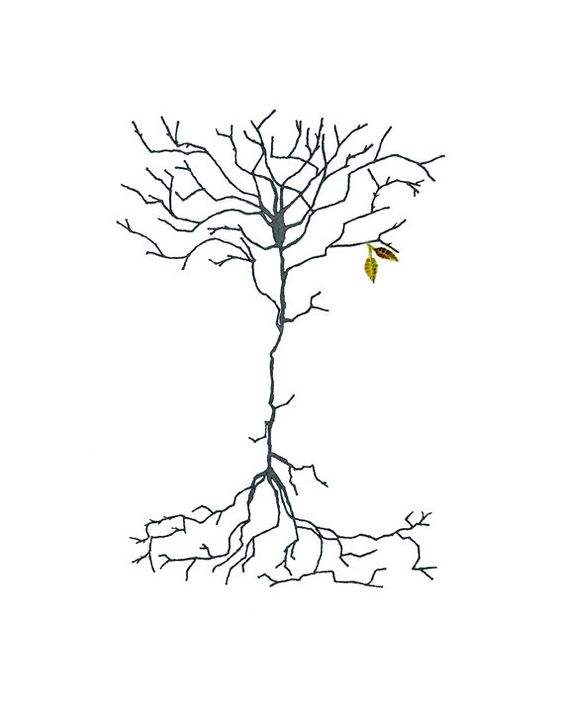
\includegraphics[height=55mm]{Figures/Cover/coverimage.jpg}  \end{center} % gr�ficos
 \vspace{5mm}
\centering
\LARGE \textbf{The spatial structure of surround modulation in mouse visual cortex}
\\ \vspace{10mm}
%\Large Subtitle
 \vspace{15mm}
\Large \textbf{Beatriz Ferreira Belbut} \\
\vspace{12mm}
\large Thesis to obtain the Master of Science Degree in
\\ \vspace{2mm}
\LARGE \textbf{Physics Engineering}
\\ \vspace{10mm}
\large Supervisors: PhD Leopoldo Petreanu and Prof. Bruno Gonçalves
\\ \vspace{15mm}
%\Large \textbf{Examination Committee}
%\\ \vspace{5mm}
%\large Chairperson:	Prof.  \\
%\large Supervisor: PhD Leopoldo Petreanu\\
%\large Co-Supervisor: Prof. Bruno Gonçalves \\
%\large Members of the Committe: Dr.  \\
%Prof. Lorem Ipsum
 
\vspace{15mm}

%\Large \textbf{\todaythesis\today} \\
\Large \textbf{October 2018} \\
\let\thepage\relax
\end{flushleft}
\pagebreak


\clearpage
% Since I am using double sided pages, the second page should be white.
% Remember that when delivering the dissertation, IST requires for the cover to appear twice.

\thispagestyle{empty}
\cleardoublepage

\setcounter{page}{1} \pagenumbering{roman}

\baselineskip 18pt % line spacing: -12pt for single spacing
                   %               -18pt for 1 1/2 spacing
                   %               -24pt for double spacingnts} 
\thispagestyle{empty}
\hbox{} \vfill
\begin{flushright}
\small \textit{\textbf{We are so familiar with seeing, that it takes a leap of imagination to realize that there are problems to be solved. But consider it. We are given tiny distorted upside-down images in the eyes, and we see separate solid objects in surrounding space. From the patterns of stimulation on the retina we perceive the world of objects and this is nothing short of a miracle.}}
\\ \vspace{2mm}  
\scriptsize Richard L. Gregory — \textit{Eye and Brain}, 1966
\end{flushright}

\clearpage
\thispagestyle{empty}
\cleardoublepage

\pdfbookmark{Acknowledgments}{Acknowledgments}
\begin{acknowledgments} 

%Leopoldo: Biology, hardware, previous software, guidance
%
%Tiago Marques: experiments, analysis, guidance
%
%Gabriela Fiorze: experiments
%
%Rhadika: Intrinsic, surgeries
%
%Oihane: Suit2p, intrinsic, surgeries
%
%Marina: surgeries
%
%Camille: surgeries
%
%Rodrigo: Tuning analysis
%
%Hedi: circuits, anatomy, connectivity
%
%all group: discussions, input, meetings, field knowledge, environment
%
%All Champalimaud comunity: CISS, posters, talks, seminars, knowledge of neuroscience
%
%Family, Francisco, friends.

\end{acknowledgments}
\clearpage
\thispagestyle{empty}
\cleardoublepage
\begin{abstract}

The Objective of this Work ... (English)

\end{abstract}
\section*{keywords}
visual neuroscience perception non-uniform asymmetry anisotropy surround modulation suppression V1 receptive field bpod spatial structure direction orientation
\clearpage
\thispagestyle{empty}
\cleardoublepage
\begin{resumo}

O objectivo

\end{resumo}
\begin{palavraschave}
Palavras-Chave
\end{palavraschave}
\clearpage
\thispagestyle{empty}
\cleardoublepage
% This is required for the fancy chapters
\dominitoc
\dominilof
\dominilot

%%%%%%%%%%%%%%%%%%%%%%%%%%%%%%%%%%%%%%%%%%%%%%%%%%%%%%%%%%%%%%%%%%%%%%
% List of contents
%\renewcommand{\baselinestretch}{1}
\pdfbookmark[0]{Index}{index}
\pdfbookmark[1]{Contents}{toc}
\tableofcontents
% \contentsline{chapter}{References}{\pageref{bib}}
\clearpage
\thispagestyle{empty}
\cleardoublepage
%\renewcommand{\baselinestretch}{1.5}
%%%%%%%%%%%%%%%%%%%%%%%%%%%%%%%%%%%%%%%%%%%%%%%%%%%%%%%%%%%%%%%%%%%%%%
% List of figures
\pdfbookmark[1]{List of Figures}{lof}
\listoffigures
\clearpage
\thispagestyle{empty}
\cleardoublepage

%%%%%%%%%%%%%%%%%%%%%%%%%%%%%%%%%%%%%%%%%%%%%%%%%%%%%%%%%%%%%%%%%%%%%%
% List of tables
\pdfbookmark[1]{List of Tables}{lot}
\listoftables
\clearpage
\thispagestyle{empty}
\cleardoublepage

% %%%%%%%%%%%%%%%%%%%%%%%%%%%%%%%%%%%%%%%%%%%%%%%%%%%%%%%%%%%%%%%%%%%%%%
% % List of algorithms
% Requires packages algorithmic, algorithm
% \pdfbookmark[1]{List of Algorithms}{loa}
% \listofalgorithms
% \cleardoublepage
\acresetall
% %%%%%%%%%%%%%%%%%%%%%%%%%%%%%%%%%%%%%%%%%%%%%%%%%%%%%%%%%%%%%%%%%%%%%%
 % List of acronyms

\pdfbookmark[1]{List of Acronyms}{loac}
%\input{acro_list}

\chapter*{Abbreviations}

\begin{acronym}[GEAI] % Give the longest label here so that the list is nicely aligned
%Note: The order matters
\acro{RF}{Receptive Field}
\acro{SM}{Surround Modulation}
\acro{V1}{primary visual cortex}
\acro{LGN}{Lateral Geniculate Nucleous}
\acro{GUI}{Graphical User Interface}
\acro{RTLSM}{Real-Time Linux State Machine}
\acro{ITI}{Inter-trial Interval}
\acro{GEAI}{Genetically Encoded neural Activity Indicator}
\acro{GECI}{Genetically Encoded Ca^{2+} Indicator}
\acro{VGCC}{Voltage-gated Ca^{2+} Channel}
\acro{ISOI}{Intrinsic Signal Optical Imaging}
\acro{TPLSM}{Two-photon Laser Scanning Microscopy}

\end{acronym}

\clearpage
\thispagestyle{empty}
\cleardoublepage




%%%%%%%%%%%%%%%%%%%%%%%%%%%%%%%%%%%%%%%%%%%%%%%%%%%%%%%%%%%%%%%%%%%%%%
% List of symbols
\pdfbookmark[1]{List of Symbols}{los}

\listofsymbols

\clearpage
\thispagestyle{empty}

\cleardoublepage
% Pages number is starting now with arabic style... until now it was on roman mode
\pagenumbering{arabic} \setcounter{page}{1}
\baselineskip 18pt
%\pagestyle{document}%Fancy head and foot with lines
\pagestyle{documentsimple}%Simple head
% %%%%%%%%%%%%%%%%%%%%%%%%%%%%%%%%%%%%%%%%%%%%%%%%%%%%%%%%%%%%%%%%%%%%%%
% The Introduction:
% %%%%%%%%%%%%%%%%%%%%%%%%%%%%%%%%%%%%%%%%%%%%%%%%%%%%%%%%%%%%%%%%%%%%%%
\fancychapter{Introduction}
\label{cap:int}

\section{A systems neuroscience question: How does the nervous system perceive the visual world?}
\label{sec:int_motivation}

Neuroscience strives to understand the organization of the nervous system, it's function and processes, as well as its relation to animal behaviour. These broad goals require a multidisciplinary integration of concepts and tools derived from biology, biophysics, anatomy, genetics, statistics, modelling, computation, ecology and psychology. Furthermore,these questions can be approached at multiple scales: from the molecular and cellular levels to the systems and neural circuits levels.

Neurons and glia, the fundamental cells in a nervous system, agglomerate in neural circuits. In the human brain, there are about $10^11$ neurons, of a great morphological and functional variety. Moreover, neurons are adaptive cells: each neurons can behave differently depending on the connections and signals it receives and transmits. 
Thus, disentangling the fundamental parameters of neuronal complexity and understanding the function of the nervous system require not only the signals and individual cell biophysical comprehension but also the understanding of the connectivity circuitry and mechanisms underlying a larger-scale neuronal network. Two systems with the same cells, arranged and interleaved with different connections would not behave equally. Correspondingly, the established knowledge on molecular and cellular neuroscience shall be integrated and complemented by a systems neuroscience approach, not as a simpler scaling step but within fundamentally different strategies. Investigating and deciphering the extraordinary questions about the nervous system in higher order completeness demand different methods, analysis and experimental paradigms than those within the study of the sum of its parts.

Neuronal systems can be described in three main functional sets: Sensory systems, motor systems and associational systems that link the former with the latter, developing more complex cognitive processes, such as perception, attention and emotions.

Animals have the enriching ability to sense the world around them. We sense our surroundings through efficiently designed stimuli sensors, and produce distinctive sensations accordingly. We are equipped with exceptionally sensible, accurate and complete input feature detectors.

However, perhaps one of the most fascinating qualities about a sensorial experience is that we can mentally encapsulate it as a given configuration and readily identify it at a future similar reoccurrence. Our nervous system allows the formation of a correspondence map between the world outside and the interior reality. The computational processing level and the efficiency of such endeavour continues to excite laborious research: How does perception arise?

In particular, the process of \textit{seeing} pertains astoundingly substantial and relevant information about the world in a remarkably efficient, fast, detailed and engaging way.

The understanding of visual perception and its processes is undertaken as one of the major withstanding challenges in systems neuroscience.

In this case, the system receives the physical image information from the retina and then parallel processes the features from the current state of the visual scene in an hierarchically organized neuronal structure. The information signals follow feedforward pathways and integrations are then carried in higher brain areas. Concurrently, feedback connections are superimposed in multiple higher order to lower order area connections, transmitting signals that underlie contextual information. Receiving this higher complexity input, neurons can then change their functioning state and produce new conjectures, educated guesses of high success probability about the input's nature. 
The unification of these parallel outputs is proposed to finally amount to a conscious sensorial perception.

There is no identity complete copy of the world outside within our perceived reality - Nonetheless, perhaps contrary to our intuition, sensitive sophisticated guesses can be just as effective, while efficient and biologically feasible within nature's parsimonious frames.

Nonetheless, fundamental questions remain for the large and complete understanding of sensory perception. In particular, discovering the computations held in the sensory cortices, their functionality, as well as the circuitry substrates that serve these mechanisms stand as main goals.

Here, we tackle a sensory neuronal property that is fundamentally implicated in visual information processing and that can yield profound insight onto the neuronal circuitry leading to visual perception - surround modulation (SM).

Neurons in the primary visual cortex (V1) respond to visual stimuli when it is presented in a given region of the visual field. For each visually responsive neuron, there is thus a \textit{receptive field} (RF) - presenting a visual stimulus of optimal parameters to that neuron in the RF corresponding visual region, will evoke a spiking response. By definition, presenting stimuli outside the RF of a neuron will amount to no response in that cell.
However, the simultaneous presentation of stimuli inside and outside the RF of a neuron will lead to a modulation of the cell's signal: the response will be either suppressed or facilitated in regards to the RF-only condition, depending on the center and surround stimuli characteristics.

This property is always active during vision processes, has been described in several species (mouse, cat, primates, humans), in various visual system areas (from the retina to the extrastriate cortex) and in multiple sensory modalities (visual, auditory, somatosensory, olfactory). A mechanistic SM theory would in this way provide a manifestly important framework in which to understand sensory processing. Moreover, understanding the circuitry that results in the SM effect and accounts for its properties can lead to insight about the function and the organization of the involved connections and network patterns - in particular, SM characterization can aid restrain circuitry models and interpret the network of inhibitory and excitatory neurons as well as feedforward, feedback and horizontal connections functionality in that perceptual integration context.

Most specifically, \textit{far} surround modulation has been suggested to require feedback input.

Typically, SM is studied in either of two methods: By using radius expanding circular grating patches or by using grating patches confined to the RF area and surrounded with annular gratings whose inner radius are made to decrease. These studies have lead to important findings about the properties of SM and elicited fruitful debate on the circuitry architectures that can result in these characteristics in a compatible way.

However, these approaches focus on static stimuli and further assume the effect's isotropy and circular symmetry. 

Recent work in mice has revealed that feedback connections from MT to V1 do not target lower-order areas irrespectively of the tuning of the higher-order sending areas. This study portrays that feedback mainly targets lower-order neurons that respond to the same positions in the visual field as the former, but that a subset of these connections are in fact dispersed to other neurons: If a higher-order neuron is tuned to a particular direction, it presents a bias to connect to a lower-order neuron that responds to the visual field positions that would appear \textit{before} in that direction line. Similarly, if a high-order neuron is orientation tuned, it presents a bias for connecting to lower-order neurons that map visual field regions at orthogonal zones to that high-order neuron's preferred orientation. 

Given the putative relation between feedback and SM, this suggested possible anisotropies in the SM effect itself, possibly to relate and to put at the perspective of the viable circuitry involved.

Here, we present an extensive characterization of SM in transgenic mice's primary visual cortex performed with two photon imaging techniques that allowed access to large datasets of differently tuned neuronal responses. We developed a moving grating stimuli presentation protocol of multiple combinations of movement directions and spatial locations that enabled the study of the spatial structure of SM and its nonuniformity.

%The mapping of moving gratings properties and the spatial structure of surround modulation can produce a set of functional rules determined in the visual cortex. It shall further provide insight into feedback mechanisms and the perception of visual scenes. 

%Precluding the project, in here we review the main related theoretical, experimental and computational topics.

%The system comprises peripheral receptors as well as central neurons. From input neurons in the retina that receive the physical image information, signals follow the visual pathway connecting to the brain, where features from the current state of the environment are parallel processed and then hierarchically repeated at higher level stages. In here, based on previously learned information of working logic inferences, the mind makes new conjectures, educated guesses of high success probability about what it is that we could be "seeing", much analogously to an extraordinarily efficient and tuned machine learning algorithm. There's no one-to-one unequivocal complete copy of the world outside within our percepted reality - But, contrary to our intuition, perhaps sensitive sophisticated guesses are just as good - as well as biologically exequivable.
%The unified binding of the parallel results of our cognition processes is presumed to amount to a conscious perception of a given state of the sensorial world.

%To investigate this complex scheme, its stages and underlying principles must be described and interpreted. 
%The purpose of this project revolves around the surround modulation effect: the finding that, if a stimulus is present in the receptive field (RF), then its surround does influence the resulting signal form of action potentials. 

%We propose the study of the spatial structure of surround modulation with motion visual scenes. This means, to analyze the effects of the location of stimuli grading patches, with varied orientations and movement directions, around the RF in the ring-shaped surround of multiple neurons of different orientation \textit{selectivity} (see section 2.2).

%Following this objective, recordings of large populations of visual cortex neurons will be obtained using two-photon microscopy in transgenic mice expressing genetically encoded calcium indicators while they observe different sets of flanking stimuli. 

%Various multidisciplinary concepts are crucial to conduct this task, and these will be motivated and exposed in the present document.

%In the following section \ref{Theoretical}, visual neuroscience main notions are described, to introduce the relevant theoretical concepts. In section \ref{Plan}, the experimental previous methods on the matter of SM are also regarded, motivating this proposal's goals and novelty. The detailed experimental procedures this project aims will then be established as to answer remaining questions about SM. This document then accounts for the relevant experimental and analytical technologies, in section \ref{Experimental}: First, an explanation is provided on behaviour measurement control settings and a programmed stimuli display protocol, as well as the further adaptations it shall undergo for this project. Secondly, the relevant principles in chemical indicators and optical physics mechanisms to use for the expression and detection of neural activity will be clarified. Finally, the analysis of the experimental data will require appropriate methods for the treatment of a large number of individual cells - We will present a possible working approach to this, Suit2p. This report will then follow with a commented bibliography, section \ref{Bib}, the calendarization of the thesis work, section \ref{Cal}, and a final discussion of the general project's plan overview, section \ref{Con}.

%\\In the following state of the art section, as a theoretical introduction, we will start by presenting visual neuroscience main general notions (section 2.1), and then specify the current understanding of the retina's neurophysiology (section 2.2) and visual cortex (section 2.3). We will then enunciate the perception organization central ideas (section 2.4) and finally review the modern surround modulation investigation results, particularizing for V1 (section 2.5).

%%other principles in neurobiology are relevant, as well as computation familiarity with Matlab, $C^{++}$, specific behavior control and measurement packages and extensions, as well as optical physics and instrumentation engineering fundaments. These will be delineated
%\\The experimental phases of this project, will be delineated starting with a section for the stimuli and software development programming (section 3.1), a review on the sort of chemical indicators, genetic manipulation and physical mechanisms used for this experiment's expression of neural activity (section 3.2) and finalized by a presentation of the recording optical technology, two-photon excitation microscopy (section 3.3).

%\\Finally, the analysis of the experimental data will require appropriate methods for the treatment of great amounts of possible parameter configurations, each for a large number of individual cells - We will present a possible working approach to this, Suit2p (section 4).

%This report will follow with a commented bibliography (section 5), the calendarization of the to-be-done work (section 6) and a final discussion of the general project's plan overview (section 7).
%\section{State of The Art}
\label{sec:int_state}

State of The Art Section.

\subsection{Dummy Subsection A}
\label{subsec:subsectiona}

State of Art Subsection A

\subsection{Dummy Subsection B}
\label{subsec:subsectionb}

State of Art Subsection B


\section{Original Contributions}
\label{sec:int_contributions}

This project can be described in two sequenced components:

\begin{itemize}
\item Stimuli display software development with bpod system for three protocols: RF mapping, tuning assessment - both adapted from the previously used bcontrol system - and SM spatial structure study. Integration of the system within the laboratory's hardware.

\item Experimental sessions with the three stimuli presentation protocols, followed by a tuning protocol validation and analytical focus on RF mapping and SM spatial structure investigations.
\end{itemize}

Within the first frame, each created protocol is made available for multiple configurations of stimuli display. The user has the flexibility to change these stimuli parameters, covering a large range of stimuli types and experimental aims.

The experimental and analytical component of the project resulted in SM spatial structure findings, for mice V1 layers 2/3. Considering that each surround patch covered a quarter-annulus around the center stimulation and that gratings could move in any of four cardinal directions:

\begin{enumerate}
\item when center and surround stimuli are simultaneously shown, there is suppression of responses in most visually responsive cells, for any stimuli configuration.
\item this suppression is significantly larger when two surround patches are displayed, instead of one (number effect).
%\item In any of the pooled conditions, going from one surround patch to two surround patches, both increased the surround 
\item there was no differential effect of SM with left versus right surround patches. The data was not conclusive for a top versus bottom surround patches effect (position effect).
\item there was a significant effect of increased suppression with shorter distances from the RF center to the surround stimuli, in the horizontal axis of the display, even whilst the cells did not respond to any of the surround-only conditions (distance effect).
\item suppression was weakly but significantly stronger for surround gratings going in the temporal direction versus going in the nasal direction. No significant difference was found for SM strength with surround gratings going in up versus down directions (direction effects).
\item Comparing surround gratings moving horizontally versus vertically held a slight but significant difference, with horizontal gratings' orientation corresponding to stronger suppression than vertical orientation (orientation effect).
\item suppression is significantly stronger when surround stimuli is presented in positions collinear to its direction of movement than when presented in flanking positions regarding that direction (alignment effect).
\item suppression is significantly stronger when presenting surround stimuli iso-directed to the center stimulus direction than when showing it cross-directed to the center stimulus direction (angle effect).
\item comparing responses from orientation selective neurons (OS), when the stimuli presented in the center was either colinear, flanking, iso-directed or cross-directed but in the preferred direction versus when in was in the anti-preferred direction yielded that suppression was significantly weaker for the former, plus the alignment and angle effects were larger. 
\item significant interactions were found between the number effect and the alignment effect, between the number effect and the angle effect and between the alignment effect and the angle effect. 
\item the variances found in the distributions of SM strength were, by quantitative order, attributable to the number effect, the preference effect, the alignment effect and the angle effect.
\end{enumerate}

In addition to these, the obtained data portrayed other trends which did not prove statistically significant. Additional data is required to discard or validate those hypothesis:

\begin{itemize}
\item surround stimuli moving towards the center stimuli versus outwards: data shows a barely significant effect for stronger suppression with the former.
\item surround stimuli and center stimuli moving in convergent versus divergent directions: data does not hold significance.
\item two surround patches moving in the same versus opposite directions to the center direction: data does not hold significance.
\end{itemize}
\section{Thesis Outline}
\label{sec:int_outline}

In the following section \ref{cap:TheoreticalIntroduction}, visual neuroscience main state of the art notions are described, to introduce the relevant theoretical concepts. 

In the technology chapter \ref{cap:Technology}, we review the chemical indicators, genetic manipulation and physical mechanisms used for this experiment's expression of neural activity, as well as the recording optical technologies, namely intrinsic signal optical imaging and two-photon excitation laser-scanning microscopy.

Chapter \ref{cap:TechnicalImplementations} describes and explains the software development phase and implemented system for stimuli display, elucidating the technical outcomes of the project.

Chapter \ref{cap:ExperimentalMethods} details the experimental methods, starting with the procedures performed with the animals, following with the visual stimulation setups for both intrinsic imaging and two-photon microscopy, then describing the experimental sessions' pipelines, stimuli presentation structure and stimuli parameters for the three protocols (RF, tuning and SM spatial structure study).

The analysis of the experimental data required appropriate methods for the treatment of great amounts of possible parameter configurations, each for a large number of individual cells. In chapter \ref{cap:Analysis}, first we enunciate the raw outputs of an experimental session and follow with the preliminary image processing stages applied to the recorded imaging data - plane separation and registration. Suit2p pipeline is then presented, as it was used for semi-automated selection of regions of interest (ROIs) to regard as neurons. Finalizing the general data treatment stages, normalized fluorescence extraction is explained. After these points, we follow with the specific analysis methods for each protocol. To conclude the chapter, we present a review on statistical notions applied for the SM data comparison analysis.

This project's results are then described in chapter \ref{cap:Results}. We start with the intrinsic optical imaging maps, follow with the general RF mapping results, tuning properties assessment and finish with the SM results analysis of individual example cells and a broader population study for SM effects.

Finally, a discussion on the findings follows in chapter \ref{cap:Discussion}, integrating the previously established SM properties across species and sensory areas with those hereby presented and contextualizing this project's results within the SM current theories. We conclude with an overall review of the project's process and enumerate potential related future work.

%In section \ref{Plan}, the experimental previous methods on the matter of SM are also regarded, motivating this proposal's goals and novelty. 

%The detailed experimental procedures this project aims will then be established as to answer remaining questions about SM. This document then accounts for the relevant experimental and analytical technologies, in section \ref{Experimental}: First, an explanation is provided on behaviour measurement control settings and a programmed stimuli display protocol, as well as the further adaptations it shall undergo for this project. Secondly, the relevant principles in chemical indicators and optical physics mechanisms to use for the expression and detection of neural activity will be clarified. Finally, the analysis of the experimental data will require appropriate methods for the treatment of a large number of individual cells - We will present a possible working approach to this, Suit2p. This report will then follow with a commented bibliography, section \ref{Bib}, the calendarization of the thesis work, section \ref{Cal}, and a final discussion of the general project's plan overview, section \ref{Con}.

%\\In the following state of the art section, as a theoretical introduction, we will start by presenting visual neuroscience main general notions (section 2.1), and then specify the current understanding of the retina's neurophysiology (section 2.2) and visual cortex (section 2.3). We will then enunciate the perception organization central ideas (section 2.4) and finally review the modern surround modulation investigation results, particularizing for V1 (section 2.5).

%%other principles in neurobiology are relevant, as well as computation familiarity with Matlab, $C^{++}$, specific behavior control and measurement packages and extensions, as well as optical physics and instrumentation engineering fundaments. These will be delineated
%\\The experimental phases of this project, will be delineated starting with a section for the stimuli and software development programming (section 3.1), a review on the sort of chemical indicators, genetic manipulation and physical mechanisms used for this experiment's expression of neural activity (section 3.2) and finalized by a presentation of the recording optical technology, two-photon excitation microscopy (section 3.3).

%\\Finally, the analysis of the experimental data will require appropriate methods for the treatment of great amounts of possible parameter configurations, each for a large number of individual cells - We will present a possible working approach to this, Suit2p (section 4).

%This report will follow with a commented bibliography (section 5), the calendarization of the to-be-done work (section 6) and a final discussion of the general project's plan overview (section 7).

\cleardoublepage
% %%%%%%%%%%%%%%%%%%%%%%%%%%%%%%%%%%%%%%%%%%%%%%%%%%%%%%%%%%%%%%%%%%%%%%
% Dummy Chapter:
% %%%%%%%%%%%%%%%%%%%%%%%%%%%%%%%%%%%%%%%%%%%%%%%%%%%%%%%%%%%%%%%%%%%%%%

% %%%%%%%%%%%%%%%%%%%%%%%%%%%%%%%%%%%%%%%%%%%%%%%%%%%%%%%%%%%%%%%%%%%%%%
% The Introduction:
% %%%%%%%%%%%%%%%%%%%%%%%%%%%%%%%%%%%%%%%%%%%%%%%%%%%%%%%%%%%%%%%%%%%%%%
\fancychapter{Theoretical Introduction}
\label{cap:Theoretical Introduction}

\textit{Present the chapter content.}

\section{Visual Neuroscience: Perception}
\label{sec:sectiona}

\section{Brain visual pathways}
\label{sec:sectionb}


\section{Receptive fields and tuning}
\label{sec:sectionb}

\section{Feedback as a path for contextual information integration}
\label{sec:sectionb}


\section{Surround modulation}
\label{sec:sectionb}

\subsection{Suppression and facilitation}
\label{subsec:subasectionE}


\subsection{Spatial structure of the phenomenon}
\label{subsec:subbsectionE}


\subsection{The motivation: feedback organization rules - uncovering the functions of feedback}
\label{subsec:subcsectionE}
\cleardoublepage

% %%%%%%%%%%%%%%%%%%%%%%%%%%%%%%%%%%%%%%%%%%%%%%%%%%%%%%%%%%%%%%%%%%%%%%
% Dummy Chapter:
% %%%%%%%%%%%%%%%%%%%%%%%%%%%%%%%%%%%%%%%%%%%%%%%%%%%%%%%%%%%%%%%%%%%%%%

% %%%%%%%%%%%%%%%%%%%%%%%%%%%%%%%%%%%%%%%%%%%%%%%%%%%%%%%%%%%%%%%%%%%%%%
% The Introduction:
% %%%%%%%%%%%%%%%%%%%%%%%%%%%%%%%%%%%%%%%%%%%%%%%%%%%%%%%%%%%%%%%%%%%%%%
\fancychapter{Technical Implementations}
\label{cap:chapter}

\textit{Present the chapter content.}

\section{Session and trial structure}
\label{sec:sectiona}



The experimental process comprised three main tasks of moving gratings stimuli viewing that were followed one next to the other in the same session.

The first protocol regarded the mapping of RF

\section{System's scheme}
\label{sec:sectionb}

\begin{figure}[H]
	\centering
		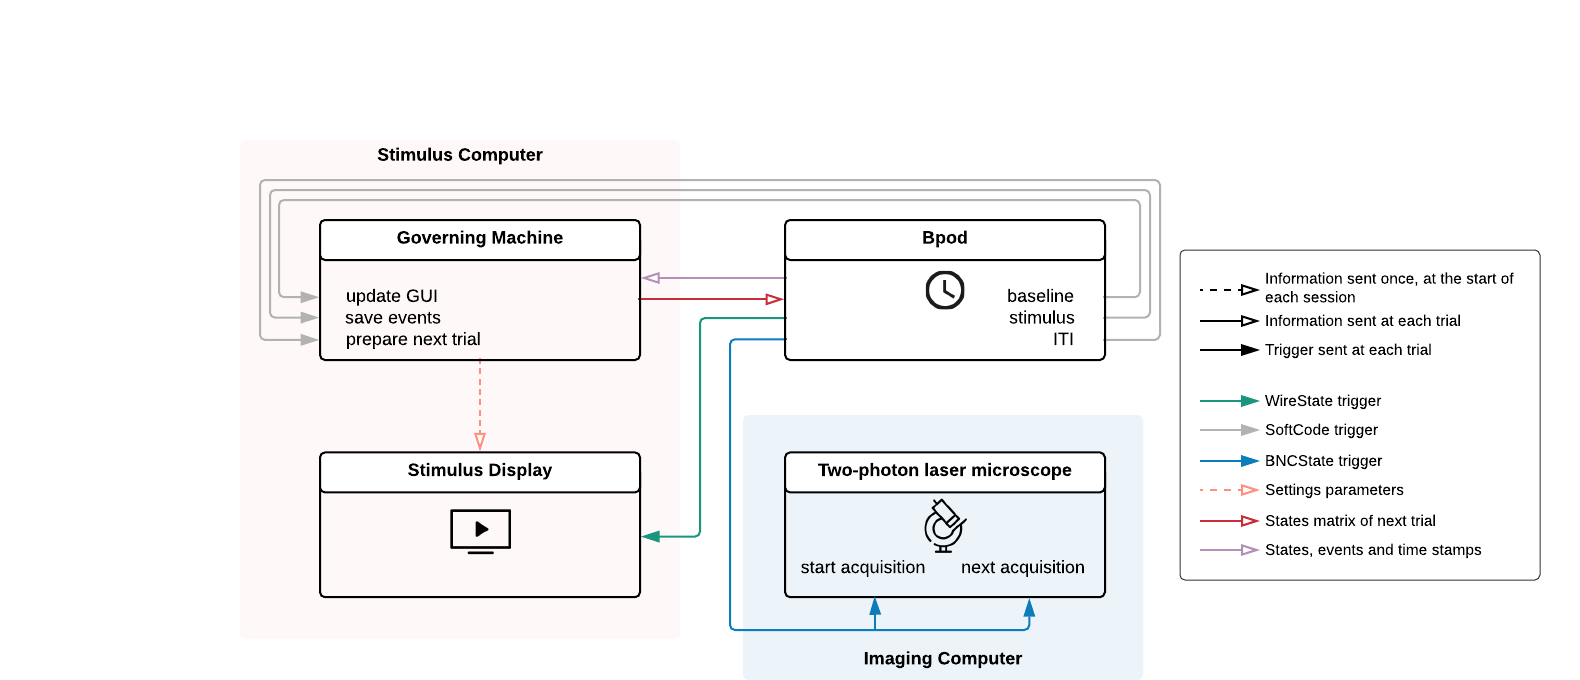
\includegraphics[width=1\linewidth]{3.Chapter/systemtechnical.png}
	\caption[c1]{Setup and connections scheme of devices used for stimuli presentation and real-time imaging.}
	\label{fig:systemtechnical}
\end{figure}
\section{Bpod}
\label{sec:sectionc}
\subsection{Motivation and previous system}
\label{subsec:subasectionC}

\subsection{Implementation and hardware alterations}
\label{subsec:subbsectionC}
\section{Software: Governing machine protocols and stimulus presentation}
\label{sec:sectiond}

\subsection{Retinotopy mapping}
\label{subsec:subasectionD}

\subsection{Implementation and hardware alterations}
\label{subsec:subbsectionD}

\subsection{Surround modulation spatial structure}
\label{subsec:subcsectionD}

\subsection{Stimulus presentation with psychtoolbox}
\label{subsec:subdsectionD}

\subsection{Optical imaging with Scanimage interface}
\label{subsec:subesectionD}
\section{Hardware: Trigger wiring and two-photon microscopy}
\label{sec:sectione}

\subsection{Triggering}
\label{subsec:subasectionE}

\subsection{Two-photon laser microscopy}
\label{subsec:subbsectionE}
\section{Instrumentation}
\label{sec:sectionf}
\cleardoublepage

% %%%%%%%%%%%%%%%%%%%%%%%%%%%%%%%%%%%%%%%%%%%%%%%%%%%%%%%%%%%%%%%%%%%%%%
% Dummy Chapter:
% %%%%%%%%%%%%%%%%%%%%%%%%%%%%%%%%%%%%%%%%%%%%%%%%%%%%%%%%%%%%%%%%%%%%%%

% %%%%%%%%%%%%%%%%%%%%%%%%%%%%%%%%%%%%%%%%%%%%%%%%%%%%%%%%%%%%%%%%%%%%%%
% The Introduction:
% %%%%%%%%%%%%%%%%%%%%%%%%%%%%%%%%%%%%%%%%%%%%%%%%%%%%%%%%%%%%%%%%%%%%%%
\fancychapter{Experimental Methods}
\label{cap:chapter}

\textit{Present the chapter content.}

\section{Animals}
\label{sec:sectiona}

All procedures were approved by the Champalimaud Centre for the Unknown Ethics Committee and carried under the stipulations of the Portuguese Direção Geral de Veterinária.

Cells' somata in V1 layer 2/3 of four Thy1-GCaMP6s ?? male?? mice (?? Laboratory stock no:??) were imaged.

Prior to the experiments, once adults (?? to ?? weaks old), the mice underwent chronic window implantation surgeries. The subjects were kept under isoflurane anesthesia and ??? analgesia. Eye moisturing was insured with ophtalmic ointment (Clorocil, Laboratório Edol).
The circular craniotomy was 

%\subsection{Subsection A}
%\label{subsec:subasectionA}
\section{Intrinsic}
\label{sec:sectionb}

%\subsection{Subsection A}
%\label{subsec:subasectionA}
\section{Specifics of the protocol settings}
\label{sec:sectionc}

\subsection{Receptive Field mapping}
\label{subsec:subasectionC}

\subsection{Tunings mapping}
\label{subsec:subbsectionC}

\subsection{Surround modulation protocol}
\label{subsec:subcsectionC}
\cleardoublepage
% %%%%%%%%%%%%%%%%%%%%%%%%%%%%%%%%%%%%%%%%%%%%%%%%%%%%%%%%%%%%%%%%%%%%%%
% Dummy Chapter:
% %%%%%%%%%%%%%%%%%%%%%%%%%%%%%%%%%%%%%%%%%%%%%%%%%%%%%%%%%%%%%%%%%%%%%%

% %%%%%%%%%%%%%%%%%%%%%%%%%%%%%%%%%%%%%%%%%%%%%%%%%%%%%%%%%%%%%%%%%%%%%%
% The Introduction:
% %%%%%%%%%%%%%%%%%%%%%%%%%%%%%%%%%%%%%%%%%%%%%%%%%%%%%%%%%%%%%%%%%%%%%%
\fancychapter{Analysis}
\label{cap:chapter}

\textit{Present the chapter content.}

\section{Pre-processing images}
\label{sec:sectiona}

\subsection{Cropping}
\label{subsec:subasectionA}

\subsection{Separating planes}
\label{subsec:subbsectionA}
\section{Suit2p pipeline}
\label{sec:sectionb}

\subsection{Registration}
\label{subsec:subasectionA}

\subsection{Selection of regions of interest (ROIs)}

\subsection{ROI labelling and quality control}

\subsection{Trace extraction and spike deconvolution}
\section{Data treatement}
\label{sec:sectionc}

\subsection{Receptive field mapping}
\label{subsec:subasectionC}

\subsection{Tuning mapping}
\label{subsec:subbsectionC}

\subsection{Surround modulation protocol}
\label{subsec:subcsectionC}
\cleardoublepage
% %%%%%%%%%%%%%%%%%%%%%%%%%%%%%%%%%%%%%%%%%%%%%%%%%%%%%%%%%%%%%%%%%%%%%%
% Dummy Chapter:
% %%%%%%%%%%%%%%%%%%%%%%%%%%%%%%%%%%%%%%%%%%%%%%%%%%%%%%%%%%%%%%%%%%%%%%

% %%%%%%%%%%%%%%%%%%%%%%%%%%%%%%%%%%%%%%%%%%%%%%%%%%%%%%%%%%%%%%%%%%%%%%
% The Introduction:
% %%%%%%%%%%%%%%%%%%%%%%%%%%%%%%%%%%%%%%%%%%%%%%%%%%%%%%%%%%%%%%%%%%%%%%
\fancychapter{Results}
\label{cap:chapter}

\textit{Present the chapter content.}

%\section{Visual Neuroscience: Perception}
\label{sec:sectiona}

\cleardoublepage


% %%%%%%%%%%%%%%%%%%%%%%%%%%%%%%%%%%%%%%%%%%%%%%%%%%%%%%%%%%%%%%%%%%%%%%
% The Introduction:
% %%%%%%%%%%%%%%%%%%%%%%%%%%%%%%%%%%%%%%%%%%%%%%%%%%%%%%%%%%%%%%%%%%%%%%
\fancychapter{Conclusions and Future Work}
\label{cap:conclusions}


\section{Surround modulation remaining questions and project's plan} \label{Plan}

\begin{itemize}
\item Summarize process and important findings and contributions
\item Compare to monkeys findings
\item Compare to mice findings
\item Put at the perspective of Tiago's work
\item highlight relevance for the field
\item future directions: more data, systematic analysis, optimization of the stimulus size
\end{itemize}


Build on(From project meft):

In a cell, SM might not be isotropic and furthermore, its anisotropy may depend on the stimulus' nature, in general or relative to the regarded neuron's selectivity. However, most previous experiments on SM have been devised with circular stimuli varying in radius, assuming the effect's isotropy. The present project proposes to tackle the possible anisotropy itself.

Furthermore, so far, studies have mostly regarded individual neuron's SM properties in cat or monkey subjects. In mice, neurons with the same orientation selectivity do not lie in the same column. Neurons with different tunings are mixed. Since this thesis task will be conducted in mice, we can thus regard multiple neurons with different tunings at once, in a more complete approach.

A recent procedure has also been done with differently localized patches of gratings in the surround \cite{SManisotropy}. However, this was conducted with static stimuli, and was furthermore executed with limited stimuli configurations. Besides using moving gratings, this project's aim is to produce an extensive study on a multitude of neurons, tunings, and stimuli configurations: Only in this way can we pursue the finding of a set of more generalized and integral SM spatial structure rules.

Having these objectives in mind, experimental and analytical steps will comprise, for each mouse: 
\begin{enumerate}
    \item Imaging large populations of neurons (>1000).
    \item Measuring the neurons' receptive fields. These will be different from cell to cell. 
    \item Suiting the larger possible number of neurons, appropriate stimulus RF and surround sizes will be fixed. Only the neurons whose receptive field does not intersect the stimuli surround will be analyzed.
    \item A central stimulus will be presented. This stimulus will be a moving grating that can have 4 different cardinal directions, thus exciting different neurons, according to their selectivities. First recordings will be for only this center stimuli (4 possibilities).
    
    \item For each of these RF's stimuli displays, small patches of moving gratings will be simultaneously presented in the surround, under a variety of configurations:
    
        \subitem{Only one patch, that can be presented in 4 angular positions of the ring-shaped surround (N, E, S, W). For each of these locations, surround gratings' will have the two directions and 2 orthogonal orientations (64 possibilities).}
        
        \subitem{Two patches located around the surround. These can be located in a vertical or horizontal direction line. For each of these configurations, the patches grating can further be with the same orientation or with opposite directions - no other relative orientation will be presented (16 possibilities).}
    
    \item Control recordings will also be operated only with surround gratings, to ensure that these are not directly driving the neuron and are by definition displayed in the surround (16 possibilities).
        
    \item The large population of neurons' responses will then be analyzed, for each of these 100 possible configurations. Comparison across neurons and across configurations will then take place, as to produce a set of SM spatial structure rules and discover possible diversity and asymmetries in neurons' responses to stimuli. 
    

\end{enumerate}

Conclusions Chapter

\cleardoublepage
\cleardoublepage
\phantomsection
\addcontentsline{toc}{chapter}{Bibliography}
\bibliographystyle{IEEEtran}
\bibliography{02.biblio}
\cleardoublepage

\begin{appendices}
	\begin{appendix}
		\pagenumbering{bychapter}
		\fancychapter{Title of AppendixA}
\label{ap:a}

   
		\cleardoublepage
	\end{appendix}
\end{appendices}


\end{document}